\documentclass[a4paper]{jpconf}
\usepackage{graphicx}
%\usepackage{subcaption}

\newcommand{\GeV}{\ensuremath{\mathrm{\:GeV}}}
\newcommand{\TeV}{\ensuremath{\mathrm{\:TeV}}}

\begin{document}

\title{Trilinear Higgs boson coupling variations for di-Higgs production with full NLO QCD predictions in \texttt{Powheg}}

\author{G.~Heinrich$^1$, S.~Jones$^2$, M.~Kerner$^3$, G.~Luisoni$^1$ and L.~Scyboz$^1$}

\address{$^1$ Max-Planck-Institut f\"ur Physik (Werner-Heisenberg-Institut), F\"ohringer Ring 6, 80805 M\"unchen, Germany}
\address{$^2$ Theoretical Physics Department, CERN, Geneva, Switzerland}
\address{$^3$ Physik-Institut, Universit\"at Z\"urich, Winterthurerstrasse 190, 8057 Z\"urich, Switzerland}
\ead{gudrun@mpp.mpg.de, s.jones@cern.ch, mkerner@physik.uzh.ch, luisonig@gmail.com, scyboz@mpp.mpg.de}


\begin{abstract}
The Higgs couplings to other particles are increasingly well-measured by the ATLAS and CMS experiments. Yet there is still room for improvement in the measurement of the Higgs trilinear self-coupling $\lambda$, mainly due to the low cross-section for Higgs boson pair production. We present inclusive and differential results for the NLO QCD corrections to Higgs pair production with the full top-quark mass dependence, where the Higgs trilinear self-coupling is varied to non-SM values. The calculation of the two-loop virtual contributions has been performed numerically using CPUs and GPUs. The fixed-order calculation is supplemented by parton showering within the \texttt{Powheg-BOX-V2} event generator, and both \texttt{Pythia8} and \texttt{Herwig7} parton-shower algorithms are implemented in a preliminary study of shower effects.
\end{abstract}


\section{Introduction}

Impressive experimental constraints have been set on the Higgs boson couplings to vector bosons and heavy fermions. The Higgs potential, in contrast, leaves more room for New Physics. Despite a low cross-section, the Higgs boson trilinear self-coupling $\lambda$ can be constrained directly by Higgs pair production $pp \to hh$.
%The best experimental limit is given by ATLAS with $-5.0 < \kappa_{\lambda} < 12.1$ at $95\%$ confidence level~\cite{ATLAS-CONF-2018-043}, from a combination of $hh \to b\bar{b}b\bar{b}, b\bar{b}\tau^+ \tau^-$ and $b\bar{b}\gamma\gamma$ channels.
Higher-order corrections to Higgs pair production have been calculated at several levels of approximation. The NLO QCD corrections with the full top-quark mass dependence were only computed more recently~\cite{Borowka:2016ehy,Borowka:2016ypz,Baglio:2018lrj}. Based on a numerical evaluation of the two-loop contribution to $gg \to hh$ performed via sector decomposition, results were computed at NLO QCD for a class of extensions of the SM. 

In this work, an implementation of the NLO QCD corrections 

\section{Description of the calculation}


\section{Total and differential cross-sections for variations of the trilinear coupling}

\begin{table}[htb!]
\begin{center}
%\setlength{\extrarowheight}{3.0pt}
\begin{tabular}{| c | c | c |c|c|}
%\Xhline{2\arrayrulewidth}
\hline
&&&&\\
$\lambda_{\mathrm{BSM}}/\lambda_{\mathrm{SM}}$ & $\sigma_{\rm{NLO}}@13 \mathrm{TeV}$\,[fb]& $\sigma_{\rm{NLO}}@14 \mathrm{TeV}$\,[fb] & $\sigma_{\rm{NLO}}@27 \mathrm{TeV}$\,[fb] &K-factor@14TeV\\
&&&&\\
\hline
-1& 116.71$^{+16.4\%}_{-14.3\%}$  & 136.91$^{+16.4\%}_{-13.9\%}$& 504.9$^{+14.1\%}_{-11.8\%}$ & 1.86 \\
\hline
0& 62.51$^{+15.8\%}_{-13.7\%}$ & 73.64$^{+15.4\%}_{-13.4\%}$& 275.29$^{+13.2\%}_{-11.3\%}$& 1.79  \\
\hline 
1& 27.84$^{+11.6\%}_{-12.9\%}$ & 32.88$^{+13.5\%}_{-12.5\%}$&127.7$^{+11.5\%}_{-10.4\%}$ &1.66\\
\hline
2 & 12.42$^{+13.1\%}_{-12.0\%}$ & 14.75$^{+12.0\%}_{-11.8\%}$ &  59.10$^{+10.2\%}_{-9.7\%}$ & 1.56 \\
\hline
2.4& 11.65$^{+13.9\%}_{-12.7\%}$ & 13.79$^{+13.5\%}_{-12.5\%}$& 53.67$^{+11.4\%}_{-10.3\%}$ & 1.65 \\
\hline
3& 16.28$^{+16.2\%}_{-15.3\%}$ & 19.07$^{+17.1\%}_{-14.1\%}$ & 69.84$^{+14.6\%}_{-12.1\%}$ & 1.90 \\
\hline 
5& 81.74$^{+20.0\%}_{-15.6\%}$  & 95.22$^{+19.7\%}_{-11.5\%}$& 330.61$^{+17.4\%}_{-13.6\%}$ & 2.14 \\
\hline 
\end{tabular}
\end{center}
\caption{Total cross-sections are given for Higgs pair production at NLO QCD at (HE-)LHC for centre-of-mass energies of $\sqrt{s}=13,14$ and $27 \TeV$. The scale uncertainties are given in percent.
\label{tab:sigmatot}}
\end{table}

\begin{figure}[htb]
  \centering
    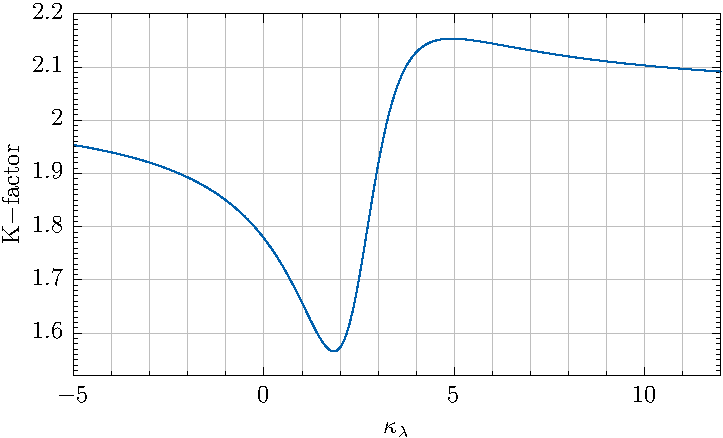
\includegraphics[width=0.65\textwidth]{plots/Kfactor.pdf}
%  \includegraphics[width=\textwidth]{plots/}
%    \caption{\label{fig:lambda_large_27}}
\caption{Variation of the NLO K-factor with the trilinear coupling at $\sqrt{s}=14$\,TeV.}
\label{fig:Kfacvariation}
\end{figure}


\begin{figure}[htb!]
\includegraphics[width=0.5\textwidth]{plots/{NLO_cHHH_1_2_2.4_0_mHH-paper}.pdf}
\hfill
    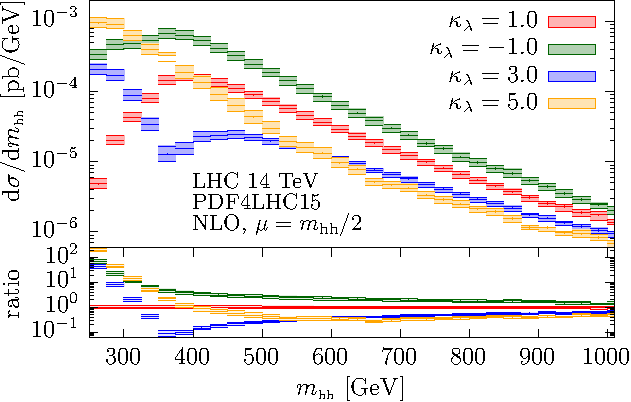
\includegraphics[width=0.5\textwidth]{plots/NLO_cHHH_1_-1_3_5_mHH-paper.pdf}
%\caption{Higgs boson pair invariant mass distributions for various
 % values of $\chhh$  at $\sqrt{s}=14$\,TeV. The uncertainty bands are from
 % scale variations as described in the text.}
\end{figure}
%\label{fig:lambdavar14TeV}

\begin{figure}[htb!]
\includegraphics[width=.45\textwidth]{plots/{NLO_PP8_PH7_PH7D_cHHH_1_ptHH}.pdf}
\hfill
    \includegraphics[width=.45\textwidth]{plots/{NLO_PP8_PH7_PH7D_cHHH_1_dRHH}.pdf}
%\caption{The transverse momentum of one (any) Higgs boson and the $R$-separation between 
%%the two Higgs bosons are shown for the fixed-order NLO calculation and three shower setups, in 
%the $\chhh=1$ case.}
\end{figure}
%\label{fig:lambdavar14TeV_pTHH_dRHH_showers}

\section{Conclusion}

\section*{References}

\bibliographystyle{iopart-num}
\bibliography{acat}{}

\end{document}


